\chapter{\uppercase{PROSPECT Analysis Framework and Calibration}}

Events in the PROSPECT detector begin as bursts of scintillation in the liquid scintillator. 
In order to transform these events of light into physics data several steps have to be taken, including position reconstruction and energy calibration. 
This chapter will outline how these processes are performed, but before that is done a key component of the PROSPECT analysis, pulse shape discrimination, must be presented.

\section{Pulse Shape Discrimination}

Physics events in the PROSPECT detector, such as neutron captures on $^6$Li, produce scintillation light through ionization that is transported by way of the reflecting panels to individual PMTs. 
As described in Section~\ref{sec:DAQ}, these signals are processed by CAEN waveform digitizers and are only accepted if they pass the segment and ZLE thresholds.
Due to the nature of the liquid scintillator the shape of the digitized waveforms is defined by the ionization density of a given event.
Lower ionization density events, such as electrons, have a faster scintillator decay time causing less light in the ``tail" of the waveform compared to higher density events like proton recoils, as seen in Figure~\ref{fig:psddefine}. 

This allows the definition of a pulse shape discrimination (PSD) factor as the ratio of the signal in the tail versus the total waveform,
\begin{equation}
	PSD =  \frac{\int_{tail:start}^{tail:end}Qdt}{\int_{-\infty}^{\infty}Qdt}
\end{equation}
The tail area of a given waveform is defined as the window 44 - 100 ns after the time of the half-height leading edge. 
The total area is defined as the window -12 - 100 ns relative to the same leading edge time. 
An example of these windows on a typical pulse can be seen in Figure~\ref{fig:psddefine}.
Use of the PSD parameter, along with energy, provides clear separation between neutron captures on $^6$Li and other event classes such as electron recoils. 
An example of this for a single segment can be seen in Figure~\ref{fig:psdvss}, where a pseudo-energy is calculated using the integrated pulse area of each PMT, S$_0$ and S$_1$.

\begin{figure}[t]
	\centering
	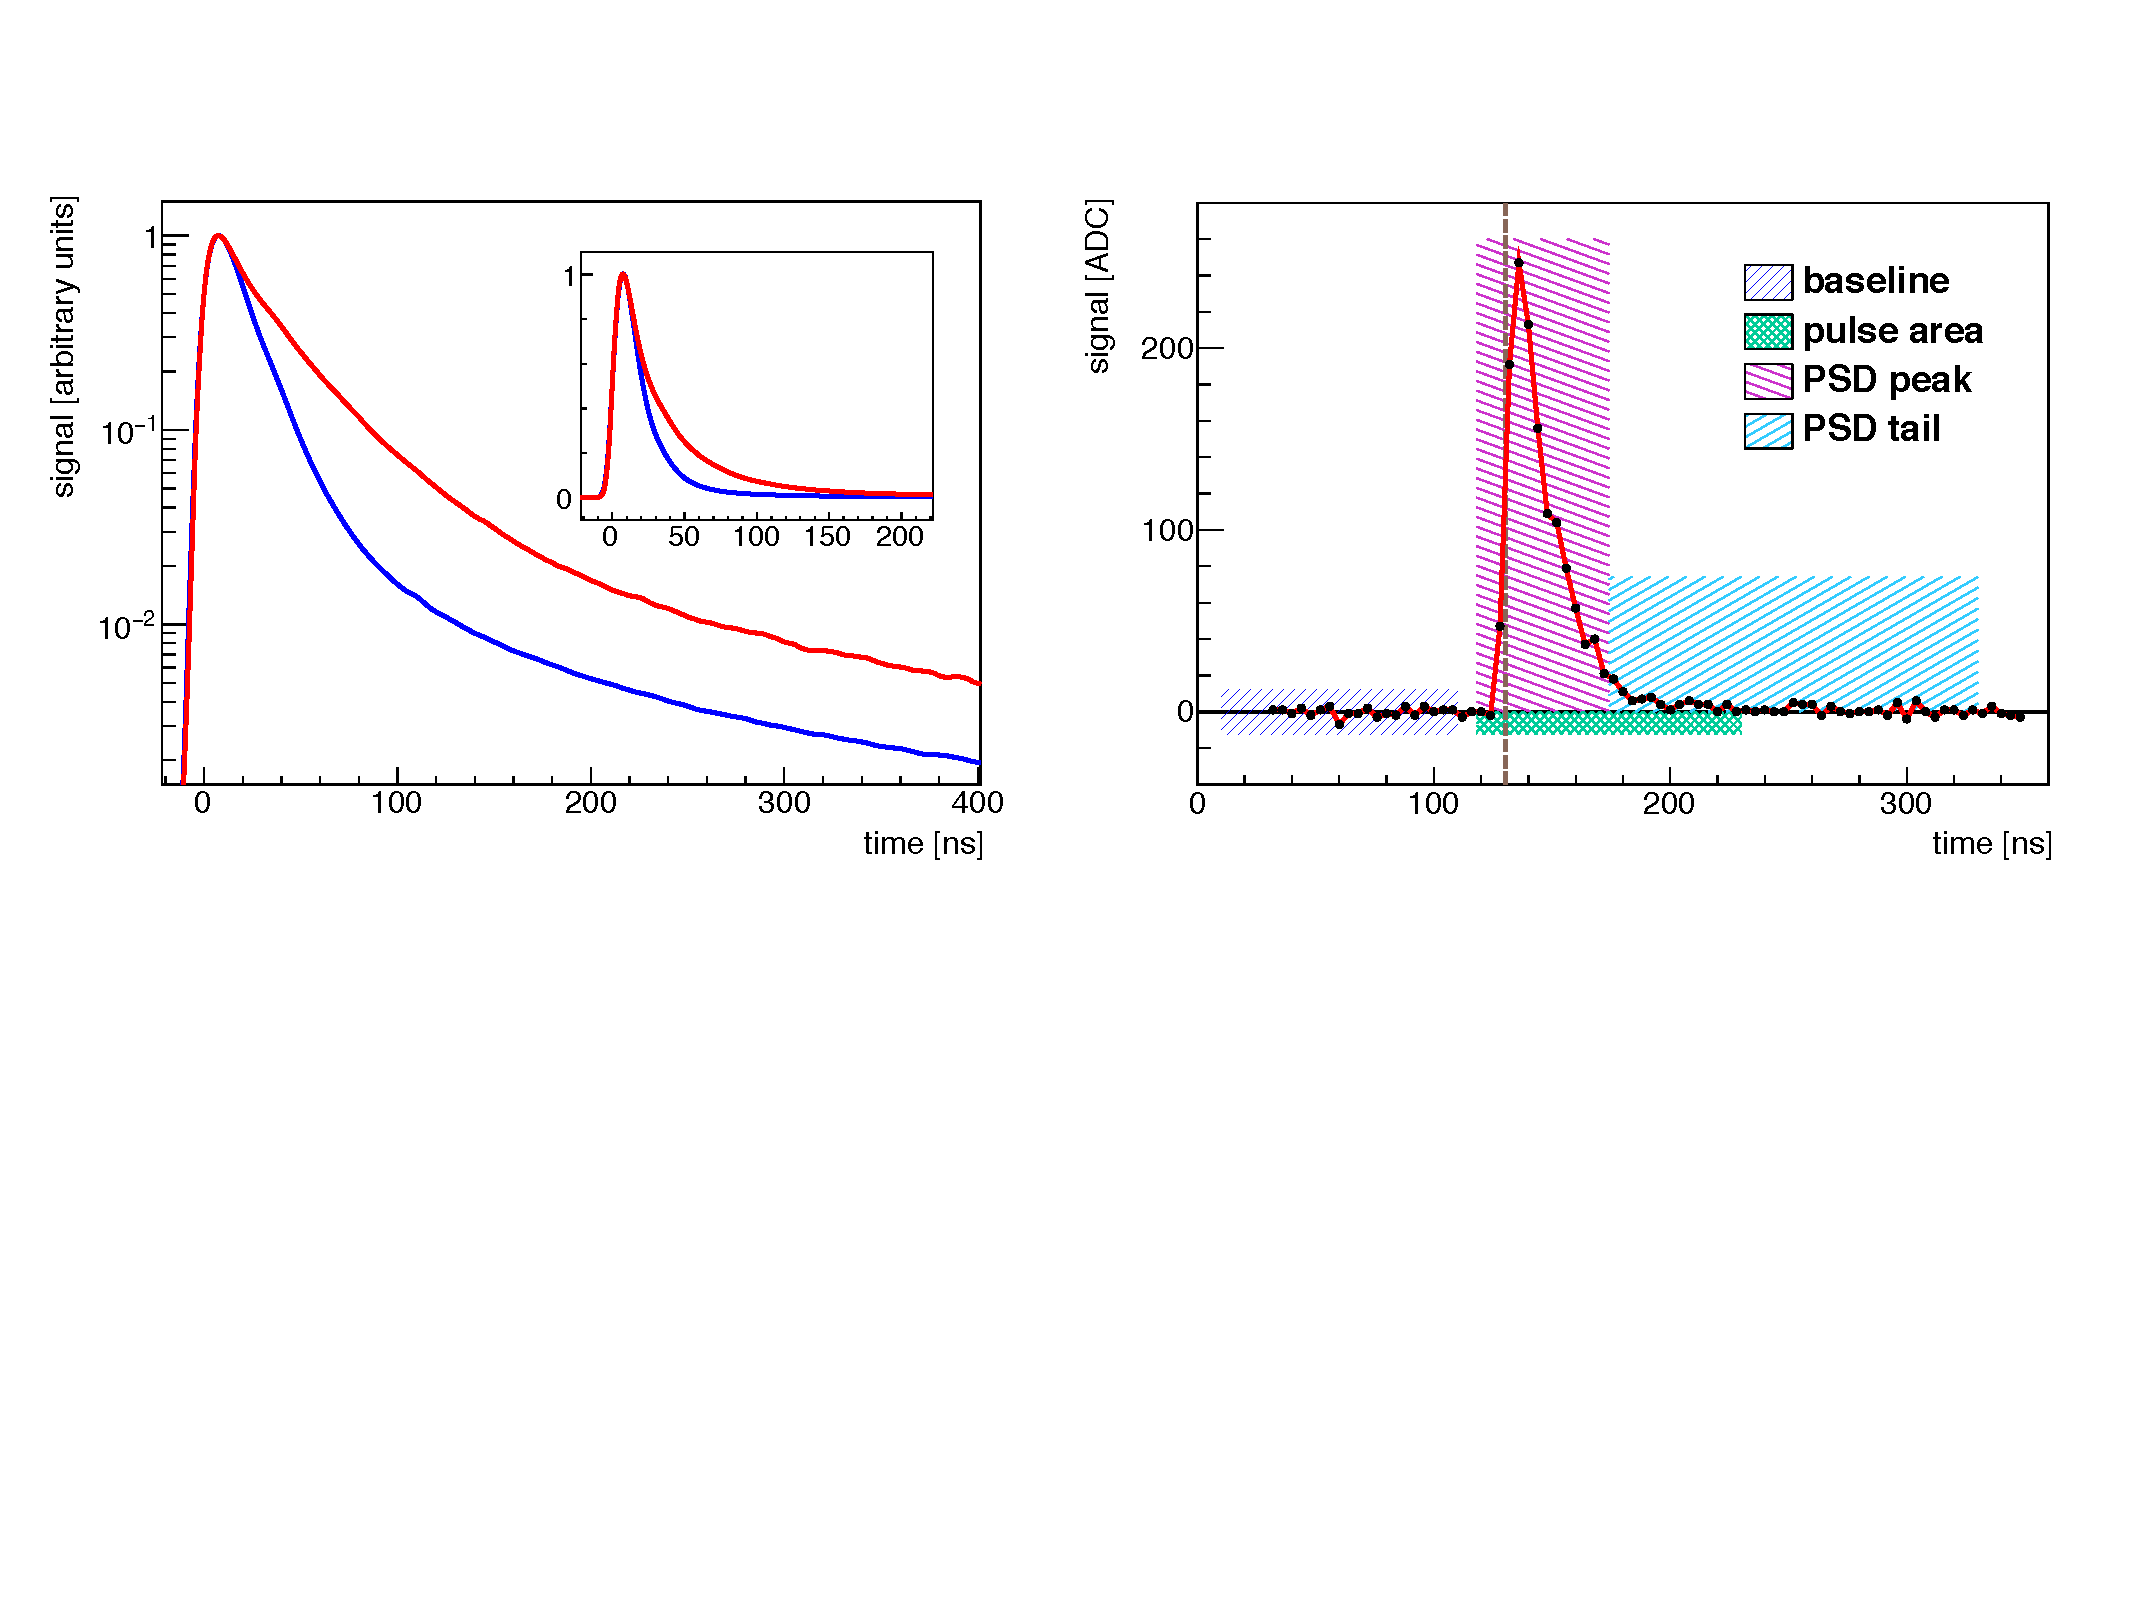
\includegraphics[width=0.99\linewidth]{tex/5-analysis-images/PSD_Define}
	\caption[Typical waveform]{(Left) Averaged waveforms from electrons (lower, blue) and proton recoils (upper, red) \cite{MM:2773}. The inset panel shows the same waveforms on a linear y axis. (Right) Example analysis of a typical pulse \cite{MM:2764}. The half-height leading edge timing (dashed vertical) determines windows for baseline subtraction, pulse area, and PSD. }
	\label{fig:psddefine}
\end{figure}

\begin{figure}[h]
	\centering
	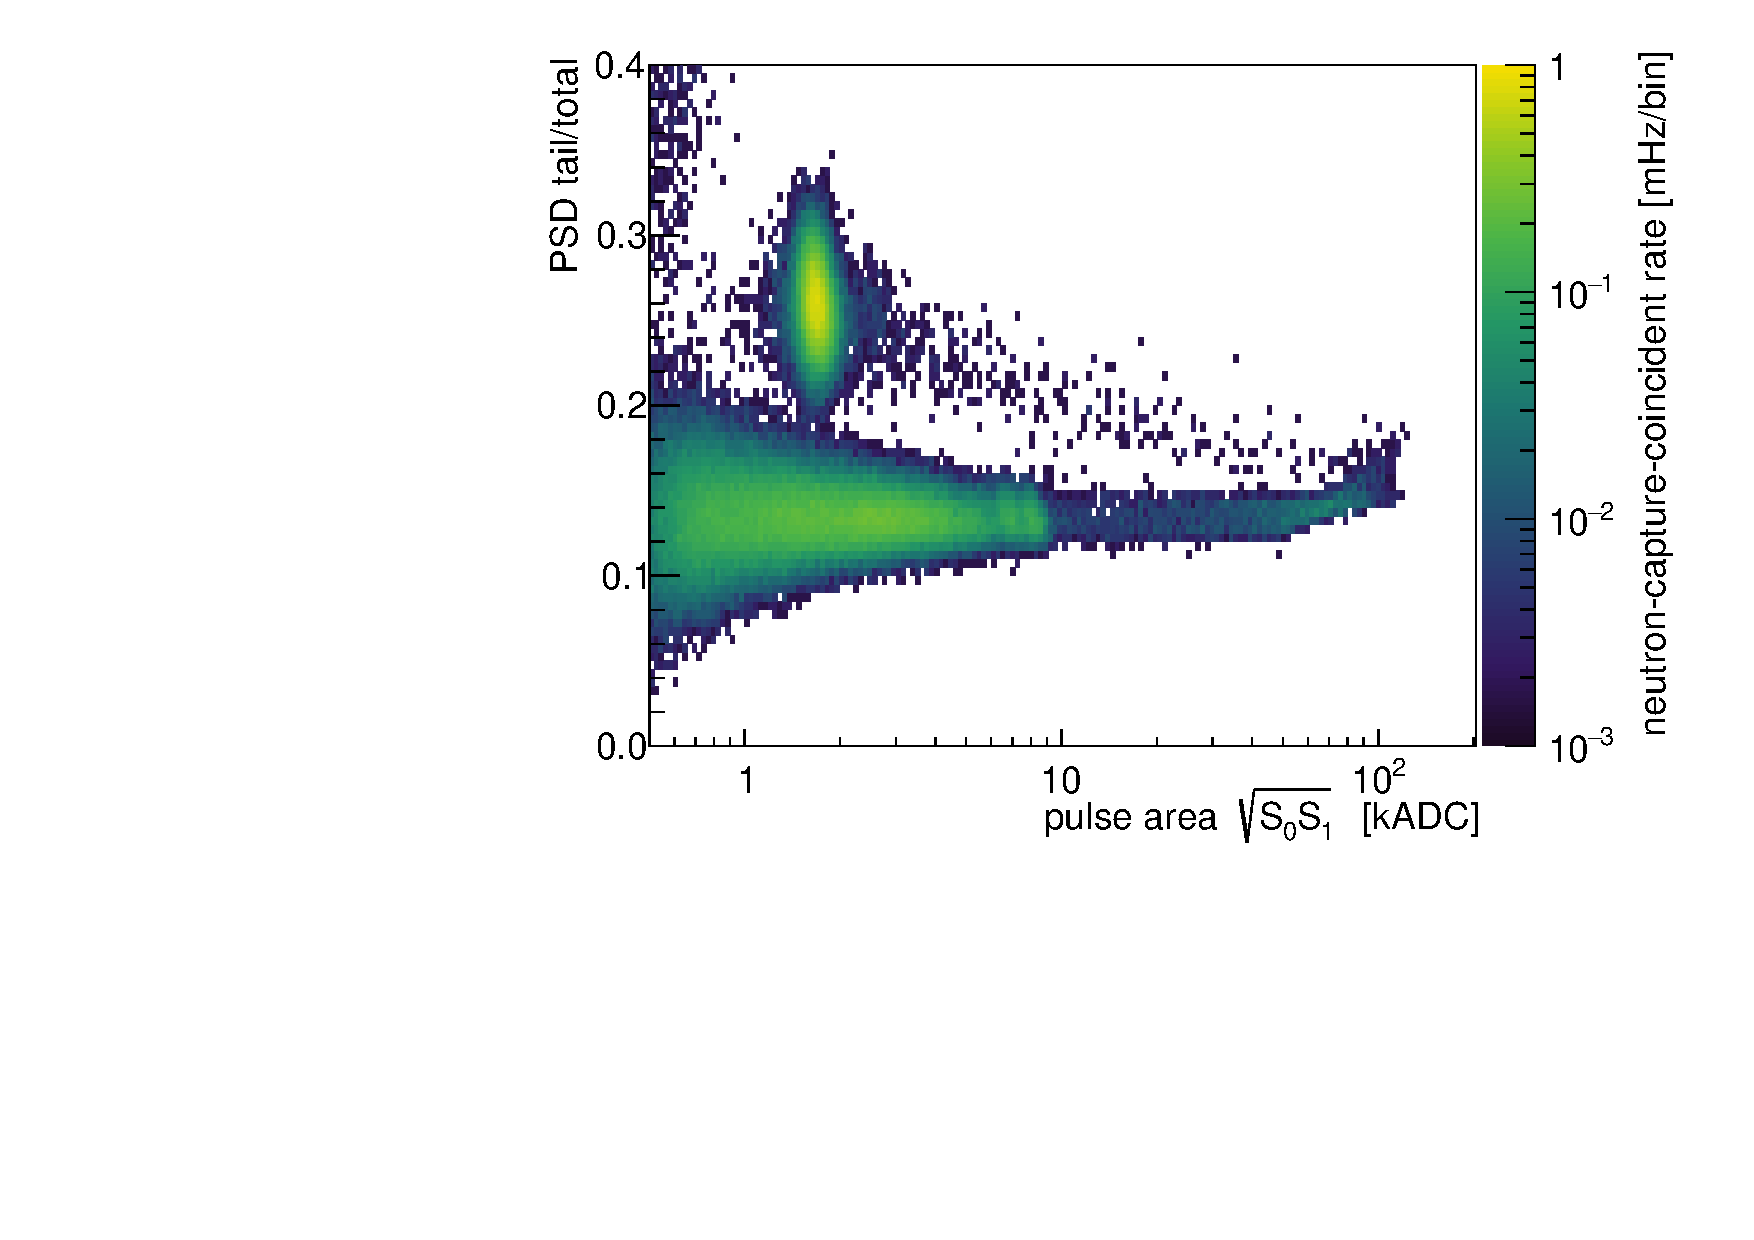
\includegraphics[width=0.6\linewidth]{tex/5-analysis-images/PSD_vs_S}
	\caption[PSD vs. psuedo-energy for neutron coincident events]{PSD vs. pseudo-energy for neutron capture coincident events in a single segment \cite{MM:2731}. The neutron captures, outlined by the magenta rectangle, are clearly separated in PSD from electron-like events in the lower band.}
	\label{fig:psdvss}
\end{figure}


\section{From Waveform to Physics Event}



